\noindent
Before moving on, I want to briefly describe what I mean by a sequencer/synthesizer/sampler, 
and also what a digital audio workstation---aka DAW---is. 

\subsection{Synthesizer}
\noindent
What I mean by a synthesizer instrument, is something that generates and plays a sound---creates audio-frequency
air pressure waves---on demand. So, when you press a key on the synthesizer's input controller, the 
synthesizer will generate---aka synthesize---and play a sound, corresponding to what key was pressed. For 
example, a basic sawtooth synthesizer is a synthesizer that creates the sawtooth wave sound on demand, 
its frequency---aka pitch---depending on which key is played on the keyboard connected to it. Pressing the 
key corresponding to the pitch A5, will result in the synthesizer synthesizing and playing a sawtooth 
wave sound at 880Hz. 

\subsection{Sampler}
\noindent
A sampler instrument, in my understanding, is actually very similar, except that instead of generating a new sound, 
it will take an existing sound---e.g. the wave format recording of a real-life snare drum being hit---and 
play it back on demand; possibly also modifying or processing it before playing it back. For example, pressing 
one key might play back the snare drum recording in its original form, literally re-playing the original wave 
recording. While pressing another key might play back the recording at half its sample rate, resulting in 
the same sound but lowered one octave.

\subsection{Sequencer}
\noindent
At the core of both these instruments are their respective input controllers; 
typically used by the human body, whether that be through hitting it, blowing air into it, stepping on it, etc.
The sequencer then, in my understanding, gets its name from the idea from an instrument that can be played, not by 
hitting it directly, but by providing it a sequence of instructions on what keys the instrument should press for 
itself, and when and in what order.

An example of such an instrument is the player piano\footnote{\url{https://en.wikipedia.org/wiki/Player_piano}},
which reads the desired keys to be pressed from a sheet of paper, written by a human who punches holes in the paper 
corresponding to the keys they want the instrument to press, and when they should be pressed. In essense, like how 
early computers were programmed, through punch cards. Presumably, because the sheets of player piano paper could get 
very long, they would be rolled up, giving them their name; piano rolls\footnote{\url{https://en.wikipedia.org/wiki/Piano_roll}}. 

A sequencer then, in my understanding, is the machine a human would use to write the program---e.g. 
a piano roll---that will then be loaded by an instrument that can understand this program; in this 
case, a player piano.
Perhaps the most common type of sequencer, fittingly, is based off the piano roll. In REAPER\footnote{\url{https://www.reaper.fm}} 
for example, the ``piano roll'' mode of its sequencer is the default mode (fig. \ref{fig:reaper_piano_roll}). 
Other modes include the ``musical notation'' mode, which is based off the Western Art or classical 
music tradition of sheet music (fig. \ref{fig:reaper_music_notation}).

\subsection{Digital audio workstation}
\noindent
A typical DAW then, is an application that combines all of the above---sequencer/synthesizer/sampler---alongside 
many other features useful for professionals and experienced hobbyists. 
For example, a DAW like the aforementioned REAPER will also allow you to record audio through it; the 
recording can then of course be played back though its sampler. Note that because the sampler is also an 
instrument, the timing of playback can also be sequenced through the included sequencer. And, though 
it comes with pre-installed instruments, third-party instruments can also be used with its sequencer, 
through integration with software instrument standards like the VST\footnote{\url{https://en.wikipedia.org/wiki/Virtual_Studio_Technology}}.

\begin{figure}[t]
	\centering
	\begin{subfigure}[b]{0.48\columnwidth}
		\centering
		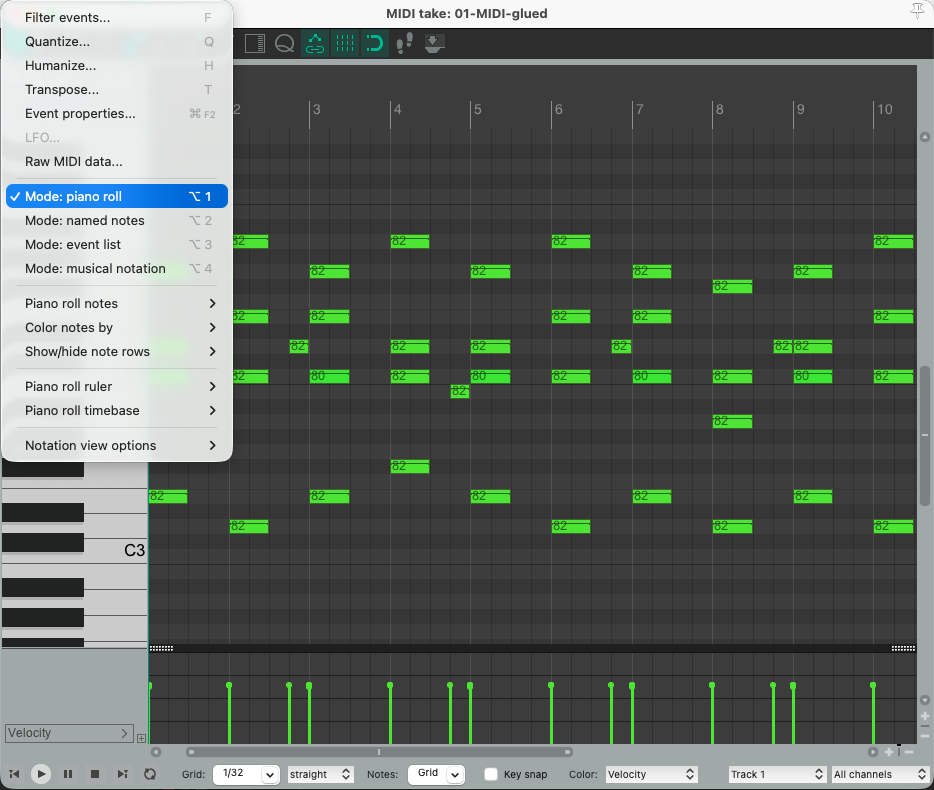
\includegraphics[width=\linewidth]{images/reaper-piano-roll}
		\caption{Piano Roll}
		\label{fig:reaper_piano_roll}
	\end{subfigure}
	\hfill
	\begin{subfigure}[b]{0.48\columnwidth}
		\centering
		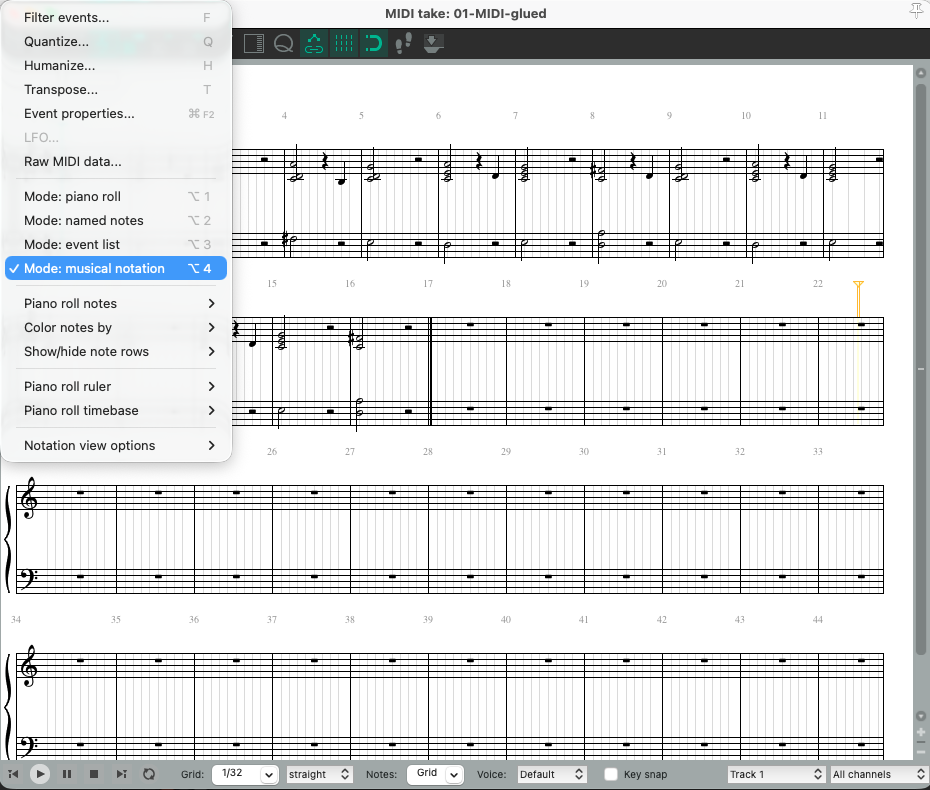
\includegraphics[width=\linewidth]{images/reaper-musical-notation}
		\caption{Musical Notation}
		\label{fig:reaper_music_notation}
	\end{subfigure}
	\caption{The modes of REAPER's MIDI sequencer}
\end{figure}
